\iffalse
\documentclass{article}
\usepackage{amsmath}
\usepackage{xcolor}
\usepackage{gensymb}
\usepackage{ragged2e}
\usepackage{graphicx}
\usepackage{gensymb}
\usepackage{mathtools}
\newcommand{\mydet}[1]{\ensuremath{\begin{vmatrix}#1\end{vmatrix}}}
\providecommand{\brak}[1]{\ensuremath{\left(#1\right)}}
\providecommand{\norm}[1]{\left\lVert#1\right\rVert}
\newcommand{\solution}{\noindent \textbf{Solution: }}
\newcommand{\myvec}[1]{\ensuremath{\begin{pmatrix}#1\end{pmatrix}}}
\let\vec\mathbf
\begin{document}
\begin{center}
        \textbf\large{CHAPTER-7 \\ TRIANGLES}
\end{center}
\section{Exercise 7.1}
Q2. \textbf{Construction}\\
\fi
\begin{figure}[H]
	\begin{center}
		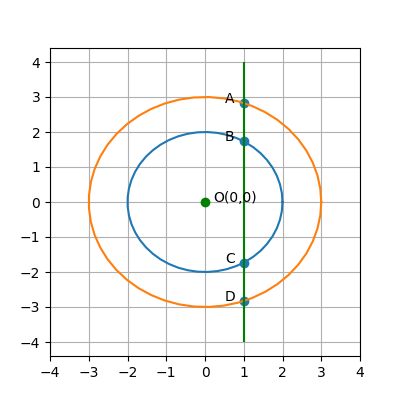
\includegraphics[width=0.75\columnwidth]{chapters/9/7/1/2/figs/fig.png}
	\end{center}
	\caption{Quadrilateral ABCD}
	\label{fig:chapters/9/7/1/2/Fig}
\end{figure}
The input parameters for construction are shown in \tabref{tab:chapters/9/7/1/2/Table1}
\begin{table}[H]
    \centering
    \begin{tabular}{|p{3cm}|p{3cm}|p{3cm}|}
\hline                                        
\textbf{Symbol} & \textbf{Values} & \textbf{Description}\\                                          
\hline                                 
$\theta$ & 30$\degree{}$   & $\angle{BAD} = \angle{BAC}$ \\           
\hline                                    
a &  9 & $AB$ \\     
\hline                      
c & 5 & $AC$ \\
\hline                                     
		$\vec{e}_1$ & $\myvec{
			1\\
			0\\
			}$ & basis vector\\ 
\hline
\end{tabular}

    \caption{Parameters}
    \label{tab:chapters/9/7/1/2/Table1}
\end{table}
Let
\begin{align}
\vec{A} =& \myvec{0\\0},\vec{B} = \myvec{a\\0},\vec{C} = \myvec{c\cos\theta\\c\sin\theta},\vec{D} = \myvec{-c\cos\theta\\c\sin\theta}
\end{align}
\begin{align}
	AB: 	\vec{n}^{\top}\vec{x} = 0,\\
\end{align}
where
\begin{align}
\vec{n} = \myvec{1\\0}
\end{align}
  From the above assumptions, we get the coordinates of $C$ and $D$ as
  \begin{align}
\vec{C} =& \myvec{4.3\\-2.5},\vec{D} = \myvec{-4.3\\-2.5}
  \end{align}
Let 
    \begin{align}
\theta_1=&\angle ADB
    \end{align}
    Since
    \begin{align}
\vec{m_1}&=\vec{D}-\vec{A}=\myvec{-4.7\\-2.5}, \vec{m_2}=\vec{D}-\vec{B}=\myvec{-13.7\\-2.5}\\
\theta_1&=\cos^{-1}\frac{\vec{m_1}^\top\vec{m_2}}{\norm{\vec{m_1}}\norm{\vec{m_2}}}\\
&=\cos^{-1}\frac{\myvec{-4.7&-2.5}\myvec{-13.7\\-2.5}}{(9.2)(15.8)}=61\degree 
\label{eq:chapters/9/7/1/2/1}
    \end{align}
    Similalrly, letting
    \begin{align}
	    \theta_2&=\angle ACB,\\
\vec{n_1}&=\vec{C}-\vec{A}=\myvec{4.7\\-2.5}, \vec{n_2}=\vec{C}-\vec{B}=\myvec{13.7\\-2.5}\\
\theta_2 &=\cos^{-1}\frac{\vec{n_1}^\top\vec{n_2}}{\norm{\vec{n_1}}\norm{\vec{n_2}}}\\
&=\cos^{-1}\frac{\myvec{4.7&-2.5}\myvec{13.7\\-2.5}}{(9.2)(15.8)}=61\degree 
\label{eq:chapters/9/7/1/2/2}
\end{align}
From \eqref{eq:chapters/9/7/1/2/1} and \eqref{eq:chapters/9/7/1/2/2},
\begin{align}
\angle ABD = \angle CAB 
\end{align}
Since all the angles and sides of triangles $CAB$ and $CAD$ are equal,
\begin{align}
    \triangle{ACB} & \cong \triangle{ADB}
\end{align}
